\section{Overview}

\subsection{Roadmap\label{sec:roadmap}}

Let us start with Composable's roadmap shown in Fig.~(\ref{fig:roadmap}) covering tasks we target to complete through the first half of 2022.
%
\begin{figure}
    \centering
    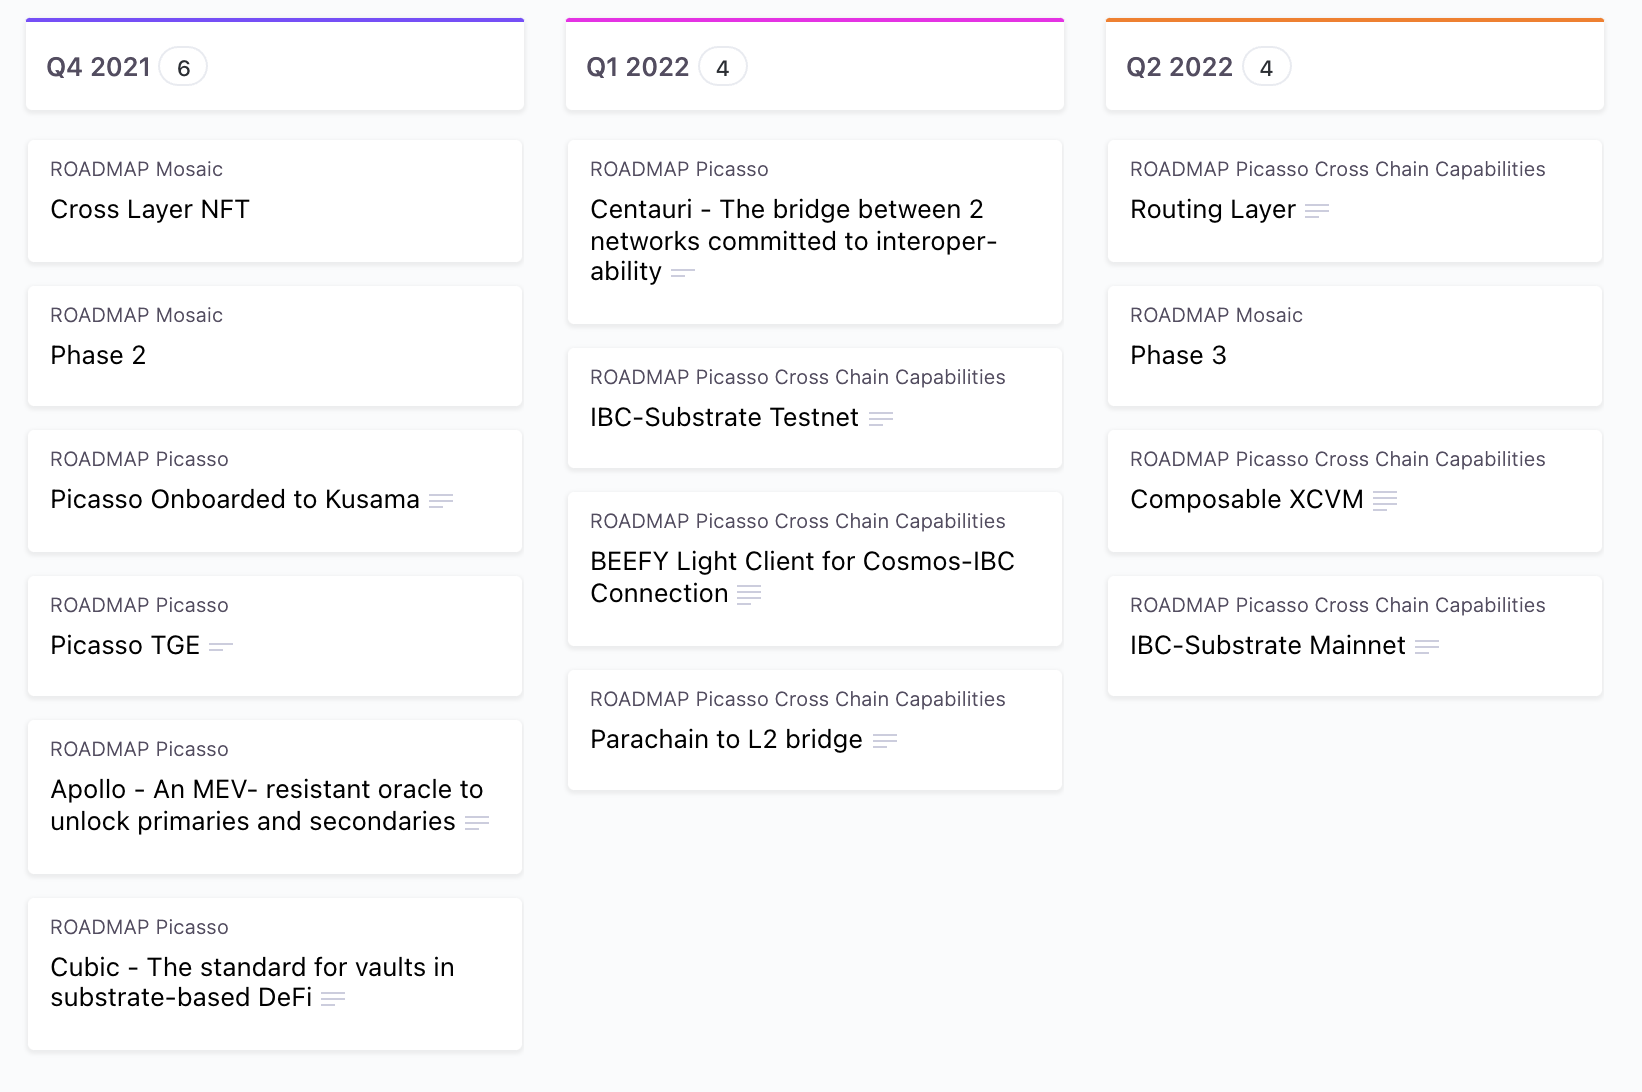
\includegraphics[width=0.9\textwidth]{images/roadmap.png}
    \caption{Composable's roadmap through first half of 2022.\label{fig:roadmap}}
\end{figure}
%
In the closing of this year, we target to enable support for cross-layer NFTs, we deploy Phase II for Mosaic, we have Picasso onboarded to Kusama.
%
The Picasso Token Generation Event (TGE) is planned to take place as well and our Oracle pallet Apollo is set to unlock primaries and secondaries.
%
We are also set to release cubic - our pallet supporting vaults known from Ethereum but in the substrate-based Polkadot and Kusama ecosystems.

In 2022, we release Centauri, the IBS Substrate testnet, we finish our developments of the BEEFY light client, and develop our Parachain to L2 bridge capability.
%
Later in that year, we finalize our routing layer and move Mosaic to Phase III which addresses decentralization. We also release our cross chain virtual machine and the IBC Substrate moves to mainnet.
%
Each of these deliverables are covered in more detail throughout this paper.

\subsection{Paper outline}

Having covered the vision in Sec.~(\ref{sec:vision}) and the roadmap in Sec.~(\ref{sec:roadmap}), we now take a look at Composable's tech stack in a top-down approach and specify in which sections throughout the Construction Paper one can find further information.

First, our Application Layer abstracts away high-level actions such as ``take out a loan on chain W layer X, then stake that on chain Y layer Z", in fact, we can get more abstract and say ``take out a loan at the lowest rate and buy NFT X" where ``X" does not include any specification of the chain or layer it lives on.
%
Much like the application Zoom, e.g., on a Mac can sync and communicate with Zoom on a PC via the internet the user needs not understand anything about the details of how the internet works (besides how to connect in the first place), they are purely seeing the abstraction of complicated information transfers underneath, at this application layer.
%
An application, however, in our case could be lending out money, taking a loan, committing capital to high-yield strategies, etc.

Let us descend one layer. We believe that the application needs to be developed in an easy to use language for developers which is blockchain agnostic. This can help bring to life the full network effect and speed of Web3.
%
This is where the Cross-Chain Virtual Machine (XCVM) comes in, see Sec.~(\ref{sec:xcvm}). In other words, XCVM is a virtual machine (akin to that familiar from Ethereum) capable of running smart contracts without the need to worry about the underlying chain-connection details.
%
XCVM, in turn, needs to send information between various blockchains and layers.
%
This is where the next layer down comes into focus: The Routing Layer, see Sec.~(\ref{sec:routing}). This is how the encoded information from developers are turned into information being sent and received to and from the relevant parties.
%
In other words, the Routing layer is responsible for routing the information from the XCVM to the correct blockchain and the correct layer, much like Port Control Protocol \cite{PortWikipedia} from Web2.

To accomplish this, the Routing Layer, in turn, needs broad access to the ecosystem of blockchains. And it needs this access to be fast and secure.
%
We have now arrived at our core layer: The Picasso Parachain for Kusama in Sec.~(\ref{sec:parachain}).
%
Incidentally, a goal is to also deploy, in a similar way, to a Polkadot parachain.
%
The parachain ensures security and speed as the applications transmit information around the entire ecosystem.

Taking a look now at the various existing ecosystems, for Ethereum we built Mosaic, covered in Sec.~(\ref{sec:mosaic}). Mosaic is a cross-layer bridge and allows for easy cross-layer transfers of tokens.
%
Mosaic is actively being built to support cross-chain transfers as well - via Picasso. To achieve our vision for Mosaic we broke down the development into three distinct phases which we will highlight here.
%
In Mosaic's Phase I, Sec.~(\ref{sec:phaseI}) aka the proof-of-concept (PoC), assets can be locked on the source layer, a relayer transmits the transferal information to the destination layer and the same amount in fees is released on the destination layer.
%
In Mosaic's Phase II, Sec.~(\ref{sec:phaseII}), we now connect multiple layers and provide multiple ways to provide liquidity on both L1 and L2. We build a software environment, Sec.~(\ref{section:lse}), to help us decide on liquidity rebalancing and an optimal fee model to use, Sec.~(\ref{sec:feemodel}).
%
In Mosaic's Phase III, Sec.~(\ref{sec:phaseIII}) we seek to increase as much as possible the decentralization of the entire system.

Next, besides Ethereum, we are also actively developing in the Polkadot and Cosmos ecosystems \cite{Cosmos:Blockchains}.
%
For Polkadot, we are creating a blockchain in Substrate \cite{HomeSubstrate_} and for Cosmos we are contributing to the Cosmos SDK.
%
Then, pallets \cite{TheMedium} are used to add additional functionality - one example is our Maximal Extractable Value (MEV) \cite{MinerEthereum.org} resistant data oracle Apollo \cite{Apollo:Finance}.
%
Other pallets can be developed including ones to enable Solidity support, cross-chain message capabilities (XCMP), decentralized exchanges, and so on.
%
Cosmos supports the Inter-Blockchain Communication Protocol (IBC) \cite{Inter-BlockchainCommunication} standard opening up for a large ecosystem that we can connect to.

In the remaining sections, we cover each of these layers in more detail and we conclude at the end in Sec.~(\ref{sec:conclusion}).
